\chapter{Cap\'{\i}tulo 3: Modelo de regresi\'{o}n ZOIP con efectos mixtos}
%{\Huge \textbf{Modelo de regresi\'{o}n ZOIP con efectos mixtos\\}}

Introduccion......

%%%%%%%%%%%%%%%%%%%%%%%%%%%%%%%%%%%%%%%%%%%%%%%%%%%%%%%%%%%%%%%%%%%%%%%%%%%%%%%%%%%%%%%%%%%%%%%%%%%%%%%%%%%%%%%%%%%%%%%%%%%%%%%%%%%%%%%%%%%%%%%%%%%%%%%%%%%%%%%%%%

\section{Modelo de regresi\'{o}n ZOIP mixto}


Una escritura jer\'{a}rquica de dos niveles considerada para un modelo con variable respuesta dada por la distribuci\'{o}n para datos proporcionales inflados con ceros y/o unos (ZOIP), vista en la secci\'{o}n \ref{Sec_dist_zoip}. Denotando a $y_{ij}$ como la $j-$\'{e}sima medida del $i-$\'{e}simo grupo, adem\'{a}s si asumisos interceptos aleatorios $\gamma_{i1}$ y $\gamma_{i2}$, los cuales son independientes y cada uno sigue una distribuci\'{o}n normal con media cero y desviaci\'{o}n est\'{a}ndar $\lambda_1$ y $\lambda_2$, respectivamente. Asumimos tambi\'{e}n que los interceptos aleatorios $\gamma_{i1}$ y $\gamma_{i2}$ son independientes entre s\'{\i}. Una escritura matem\'{a}tica para el modelo es el siguiente:

\[
y_{ij}| \gamma_{i1},\gamma_{i2} \overset{\text{ind}}{\sim} ZOIP(\mu_{ij},\sigma_{ij},p_0, p_1),
\]
\[
\gamma_{i1} \overset{\text{i.i.d}}{\sim}  N(0,\lambda_1^2),
\]
\[
\gamma_{i2} \overset{\text{i.i.d}}{\sim}  N(0,\lambda_2^2),
\]
\\
Para $i=1,2,\ldots, N$ y $j=1,2,\ldots, n_i$ Los par\'{a}metros $\mu$, $\sigma$, $p_0$ y $p_1$ son modelados linealmente en funci\'{o}n de un conjunto de covariables respectivamente, por:


\[
h_1(\mu_{ij})=\mathbf{x}_{ij1}^{\top} \boldsymbol{\beta}_1+ \gamma_{i1},
\]
\[
h_2(\sigma_{ij})=\mathbf{x}_{ij2}^{\top} \boldsymbol{\beta}_2+ \gamma_{i2},
\]
\[
h_3(p_0)=\mathbf{x}_{ij3}^{\top} \boldsymbol{\beta}_3,
\]
\[
h_4(p_1)=\mathbf{x}_{ij4}^{\top} \boldsymbol{\beta}_4
\]


donde $\mathbf{x}_{ij1}$, $\mathbf{x}_{ij2}$, $\mathbf{x}_{ij3}$ y $\mathbf{x}_{ij4}$, son vectores de covariables conocidos de dimensi\'{o}n $k_1$, $k_2$, $k_3$ y $k_4$ respectivamente. $\boldsymbol{\beta}_1$, $\boldsymbol{\beta}_2$, $\boldsymbol{\beta}_3$ y $\boldsymbol{\beta}_4$ son vectores de par\'{a}metros desconocidos fijos asociados a las covariables y $\gamma_{i1}$, $\gamma_{i2}$ son los interceptos aleatorios asociados al $i-$\'{e}simo grupo. Adem\'{a}s las funciones $h_1(\cdot)$, $h_2(\cdot)$, $h_3(\cdot)$ y $h_4(\cdot)$ son funciones de enlace conocidas y apropiadas para mapear de los reales a los valores admisibles del par\'{a}metro, ademas son funciones estrictamente mon\'{o}tonas y doblemente diferenciables. Las posibles funciones para el par\'{a}metro $\mu$ y $\sigma$ son logit, probit, clog-log, o log dependiendo de la parametrizaci\'{o}n,  para los par\'{a}metros de inflaci\'{o}n $p_0$ y $p_1$ son posibles funciones de enlace como logit, probit, clog-log.

\subsection{Inferencia estad\'{\i}stica}

La estimaci\'{o}n de los par\'{a}metros del modelo de regresi\'{o}n con intercepto aleatorio para datos proporcionales inflados con ceros y/o unos, por medio de m\'{a}xima verosimilitud, es necesario hallar la funci\'{o}n de verosimilitud.

Considere $\boldsymbol{\theta}=(\boldsymbol{\beta_1}^{\top},\boldsymbol{\beta_2}^{\top},\boldsymbol{\beta_3}^{\top}, \boldsymbol{\beta_4}^{\top},\lambda_1,\lambda_2)^{\top}$ un vector de par\'{a}metros a ser estimado en el espacio:
\[
\Theta=\left\{\boldsymbol{\theta} \in \mathbb{R}^k | \boldsymbol{\beta_1} \in \mathbb{R}^{k_1}, \boldsymbol{\beta_2} \in \mathbb{R}^{k_2}, \boldsymbol{\beta_3} \in \mathbb{R}^{k_3}, \boldsymbol{\beta_4} \in \mathbb{R}^{k_4}, \lambda_1 \in \mathbb{R}^+, \lambda_2 \in \mathbb{R}^+  \right\}
\]

en el que $k=k_1+k_2+k_3+k_4+2$, tenemos que una distribuci\'{o}n marginal de $\mathbf{y}_i=(y_{1i},\ldots, y_{n_i}i)^{\top}$ es dada por:

\[
f(\mathbf{y}_i;\boldsymbol{\theta})=\int_{\mathbb{R}^2}\prod_{j=1}^{n_i}f(y_{ij}|\gamma_{i1},\gamma_{i2};\boldsymbol{\beta_1}, \boldsymbol{\beta_2}, \boldsymbol{\beta_3}, \boldsymbol{\beta_4})\cdot f(\gamma_{i1};\lambda_1) f(\gamma_{i2};\lambda_2) d\gamma_{i1}d\gamma_{i2},
\]

Entonces una funci\'{o}n de verosimilitud para las observaciones $\mathbf{y}=(y_1, \cdots, y_N)^{\top}$ es de la forma:

\[
L(\boldsymbol{\theta})=\prod_{i=1}^{N}f(\mathbf{y}_i;\boldsymbol{\theta})
\]
\[
=\prod_{i=1}^{N}\int_{\mathbb{R}^2}\prod_{j=1}^{n_i}f(y_{ij}|\gamma_{i1},\gamma_{i2};\boldsymbol{\beta_1}, \boldsymbol{\beta_2}, \boldsymbol{\beta_3}, \boldsymbol{\beta_4})\cdot f(\gamma_{i1};\lambda_1) f(\gamma_{i2};\lambda_2) d\gamma_{i1}d\gamma_{i2},
\]

\begin{equation}
\ell(\boldsymbol{\theta})=\sum_{i=1}^{N}log \left[\int_{\mathbb{R}^2}\prod_{j=1}^{n_i}f(y_{ij}|\gamma_{i1},\gamma_{i2};\boldsymbol{\beta_1}, \boldsymbol{\beta_2}, \boldsymbol{\beta_3}, \boldsymbol{\beta_4})\cdot f(\gamma_{i1};\lambda_1) f(\gamma_{i2};\lambda_2) d\gamma_{i1}d\gamma_{i2}\right],
 \label{func_ver_mix}
\end{equation}


donde $f(y_{ij}|\gamma_{i1},\gamma_{i2};\boldsymbol{\beta_1}, \boldsymbol{\beta_2}, \boldsymbol{\beta_3}, \boldsymbol{\beta_4})$ es la funci\'{o}n de densidad de probabilidad condicional de $y_{ij}$ que distribuye $ZOIP(\mu,\sigma,p_0,p_1)$. $\gamma_{i1}$, $\gamma_{i2}$ y $f(\gamma_{i1};\lambda_1)$ y $f(\gamma_{i2};\lambda_2)$ son funciones de densidades de probabilidad normales de $\gamma_{i1}$ y $\gamma_{i2}$, respectivamente. Para encontrar el m\'{a}ximo de la funci\'{o}n $\ell(\boldsymbol{\theta})$ no es posible mediante una manera cerrada anal\'{\i}ticamente, una dificultad adicional es la soluci\'{o}n de la integral para encontrar la maximizaci\'{o}n de la funci\'{o}n $\ell(\boldsymbol{\theta})$, por lo que es necesario utilizar t\'{e}cnicas computacionales para la soluci\'{o}n de esta, t\'{e}cnicas tales como aproximaciones de Laplace, algoritmos EM, integraci\'{o}n Monte Carlo o t\'{e}cnicas bayesianas. Para solucionar dicha funci\'{o}n de log-verosimilitud utilizamos el m\'{e}todo de integraci\'{o}n num\'{e}rica Gauss-Hermite adaptativa multidimensional con y sin pruning, tal como se describe en la siguiente secci\'{o}n.


\subsection{Cuadratura de Gauss-Hermite}\label{sec:Cuadratura}

\subsubsection{Cuadratura de Gauss-Hermite unidimensional}

La cuadratura de Gauss-Hermite (GQ) es una herramienta \'{u}til para aproximar una integral de una funci\'{o}n $g(x)$ sobre $\Re$ con una suma ponderada, donde la variable $x$ es reemplazada por una cuadratura de $n$ puntos o nodos. Cada punto de la cuadratura, es denotado por $p_i$, es evaluado en la funci\'{o}n y los resultados son ponderados por los pesos de la cuadratura asociados $w_i$.
\[
\int_\Re{g(x)dx}\approx\sum_{i=1}^{n}{g(p_i)exp(p_i^2)w_i.}
\]
\\
El conjunto de los $n$ puntos de la cuadratura $\textbf{P}=\left\{p_1,p_2,\ldots,p_n\right\}$ corresponde a las ra\'{\i}ces del polinomio de Hermite dado por:

\[
H_n{(x)}=(-1)^ne^{-x^2}\frac{d^n}{dx^n}e^{-x^2},
\]
\\
con pesos asociados $\textbf{W}=\left\{w_1,w_2,\ldots,w_n\right\}$ dados por

\[
w_i=\frac{2^{n-1}n!\sqrt{\pi}}{n^2{[H_{n-1}(x_i)]}^2}.
\]

\subsubsection{Cuadratura de Gauss-Hermite adaptativa}

\textbf{Unidimensional\\}
La cuadratura de Gauss-Hermite adaptativa (AGQ) es propuesta por \cite{Liu1}; \citep{Pinheiro1}, es b\'{a}sicamente una transformaci\'{o}n de los puntos asociados a la cuadratura, centrando y extendiendo alrededor del m\'{a}ximo valor de $\hat{x}$ de la funci\'{o}n $log(g(x))$. La transformaci\'{o}n de los puntos de la cuadratura $p_i$ definido como $p_i^*$, est\'{a} dado por $p_i^*=\sqrt{2}\hat{\sigma}p_i+\hat{x}$ donde:

\[
\hat{\sigma}^2={\left[\left. -\frac{d^2}{dx^2}log(g(x))\right|_{x=\hat{x}}\right]^{-1}}.
\]
\\
As\'{\i}, la aproximaci\'{o}n de la integral de $g(x)$ sobre $\Re$ est\'{a} dado por:

\[
\int_\Re{g(x)dx}\approx\sqrt{2}\hat{\sigma}\sum_{i=1}^{n}{g(p_i^*)exp(p_i^2)w_i.}
\]

\textbf{Multidimensional\\}
Si extendemos la AGQ a una integral de dimensi\'{o}n q de la funci\'{o}n $g(x)$ sobre $\Re^q$, en este caso, con una cuadratura de $n$ puntos, $\textbf{Z}$ est\'{a} basado en el producto cartesiano de $\textbf{P}$, y los pesos de la cuadratura de $\textbf{A}$ est\'{a} basado similarmente en el producto Kronecker, denotado por $\otimes$, los pesos originales $\textbf{W}$, es dado:

\[
\textbf{Z}=\underbrace{P \times \ldots \times P}_{q\ \text{veces}}=P^q,
\]

\[
\textbf{A}=\underbrace{W \otimes \ldots \otimes W}_{q\ \text{veces}}.
\]
\\
As\'{\i}, la expresi\'{o}n para la integral aproximada de $g(x)$ sobre $\Re^q$ est\'{a} dado por:

\[
\int_{\Re^q}{g(x)dx}\approx|\hat{Q}|^{1/2} 2^{q/2}\sum_{i=1}^{n^q}g(z_i^*)exp(z_i^{\top}z_i)a_i,
\]
\\
donde $z_i$ y $a_i$ corresponde a los elementos de $\textbf{Z}$ y $\textbf{A}$, respectivamente. Los nuevos puntos de la cuadratura $z_i^*$ estan centrados en el m\'{a}ximo de $\hat{x}$ del $log(g(x))$ y est\'{a} dado por $z_i^*=\hat{x}+\sqrt{2}\hat{Q}^{1/2}z_i$, donde $\hat{Q}^{1/2}$ corresponde a la descomposici\'{o}n de Cholesky de la curvatura de la matriz $\hat{Q}$, que se encuentra dado por:

\[
\hat{Q}={\left[\left. -\frac{d^2}{dx^2}log(g(x))\right|_{x=\hat{x}}\right]^{-1}}.
\]

\subsubsection{Cuadratura de Gauss-Hermite adaptativa con Pruning}

Es claro que los resultados obtenidos por la AGQ son mejores que los de GQ, debido a que se encuentran centrados, sin embargo, la AGQ requiere un tiempo de optimizacion mas elevado, debido a la transformacion de los puntos de cuadratura, pero no todos los puntos de la AGQ aportan de manera significativa un valor sobre la solucion de la integral, es por esto que \cite{Hernandez1} desarrolla un mejoramiento de la AGQ, donde elimina los puntos de la cuadratura que no son significativos sobre la solucion de la integral, de modo que no afectan de manera significaativa los resultados finales de la integral, pero si afectan de manera positiva el tiempo de ejecucion, dicho mejoramiento es llamado cuadratura de Gauss-Hermite con pruning. 

La cuadratura de Gauss-Hermite adaptativa con pruning consiste en eliminar puntos de la cuadratura, tales que el peso $a_i$ asociado al punto es menor que un valor de referencia dado por $\theta$, que est\'{a} dado por:
\[
\theta=\frac{w_{[1]}w_{[\frac{n+1}{2}]}}{n^{q-1}}.
\]
\\
donde $w_{[1]}$ y $w_{[\frac{n+1}{2}]}$ corresponden respectivamente, a el valor minimo y la mediana de los pesos originales \textbf{W}. (Ver m\'{a}s en \cite{Hernandez1}.)


\subsection{Aproximaci\'{o}n de la funci\'{o}n de verosimilitud v\'{\i}a cuadratura de Gauss-Hermite}

En la funci\'{o}n de verosimilitud definida en \eqref{func_ver_mix} se tiene que para cada i-esimo grupo se debe resolver la siguiente integral:

\begin{align*}
I_i &= \int_{\Re^2}{\prod_{j=1}^{n_i}f(y_{ij}|\gamma_{i1},\gamma_{i2};\boldsymbol{\beta_1}, \boldsymbol{\beta_2}, \boldsymbol{\beta_3}, \boldsymbol{\beta_4})\cdot f(\gamma_{i1};\lambda_1) f(\gamma_{i2};\lambda_2) d\gamma_{i1}d\gamma_{i2}}\\
&=\int_{\Re^2}{\prod_{j=1}^{n_i}f(y_{ij}|\gamma_{i1},\gamma_{i2};\boldsymbol{\beta_1}, \boldsymbol{\beta_2}, \boldsymbol{\beta_3}, \boldsymbol{\beta_4})\cdot \frac{exp({\gamma_{i1}^2}/{2\lambda_1^2})}{\lambda_1\sqrt{2\pi}} \cdot \frac{exp({\gamma_{i2}^2}/{2\lambda_2^2})}{\lambda_2\sqrt{2\pi}} d\gamma_{i1}d\gamma_{i2}}
\end{align*}

Si se realiza el siguiente cambio de variables

\begin{equation*}
\begin{aligned}
b_{i1}&=\frac{\gamma_{i1}}{\sqrt{2}\lambda_1}\\
\therefore b_{i1}^2&=\frac{\gamma_{i1}^2}{2\lambda_1^2}\\
\therefore \gamma_{i1}&=\sqrt{2}\lambda_1b_{i1}\\
\end{aligned}
\quad
\begin{aligned}
b_{i2}&=\frac{\gamma_{i2}}{\sqrt{2}\lambda_2}\\
b_{i2}^2&=\frac{\gamma_{i2}^2}{2\lambda_2^2}\\
\gamma_{i2}&=\sqrt{2}\lambda_2 b_{i2}
\end{aligned}
\end{equation*}

Por lo anterior se tiene que la integral $I_i$ se convierte en:

\begin{equation}
I_i=\int_{\Re^2}{\prod_{j=1}^{n_i}f(y_{ij}|\sqrt{2}\lambda_1b_{i1},\sqrt{2}\lambda_2 b_{i2};\boldsymbol{\beta_1}, \boldsymbol{\beta_2}, \boldsymbol{\beta_3}, \boldsymbol{\beta_4})\cdot \frac{exp(-b_{i1}^2) exp(-b_{i2}^2)}{\pi} db_{i1}db_{i2}}
\label{Int_vero_mix}
\end{equation}

La integral definida en \eqref{Int_vero_mix} tiene una forma factible para ser aproximada usando la cuadratura de Gauss-Hermite adaptativa multidimensional con o sin pruning, vista en la secci\'{o}n \ref{sec:Cuadratura}, de este modo la integral $I_i$ es aproximada por:

\[
I_i=\sum_{k_1=1}^{Q_1}{\sum_{k_2=1}^{Q_2}{\prod_{j=1}^{n_i}f(y_{ij}|\sqrt{2}\lambda_1 z_{k_1},\sqrt{2}\lambda_2 z_{k_2};\boldsymbol{\beta_1}, \boldsymbol{\beta_2}, \boldsymbol{\beta_3}, \boldsymbol{\beta_4})\cdot \frac{w_{k_1}w_{k_2}}{\pi}}}
\]

donde $z_{k_1}$ y $z_{k_2}$ son los puntos de la cuadratura, $w_{k_1}$ y $w_{k_2}$ son los pesos asociados a los puntos de la cuadratura, por lo tanto la funci\'{o}n de verosimilitud aproximada es dado por:

\[
L(\boldsymbol{\theta})=\prod_{i=1}^{N}{\left[\sum_{k_1=1}^{Q_1}{\sum_{k_2=1}^{Q_2}{\prod_{j=1}^{n_i}f(y_{ij}|\sqrt{2}\lambda_1 z_{k_1},\sqrt{2}\lambda_2 z_{k_2};\boldsymbol{\beta_1}, \boldsymbol{\beta_2}, \boldsymbol{\beta_3}, \boldsymbol{\beta_4})\cdot \frac{w_{k_1}w_{k_2}}{\pi}}}\right]}
\]

y la funci\'{o}n de log verosimilitud esta dado por:

\begin{equation}
\ell(\boldsymbol{\theta})=\sum_{i=1}^{N}log{\left[\sum_{k_1=1}^{Q_1}{\sum_{k_2=1}^{Q_2}{\prod_{j=1}^{n_i}f(y_{ij}|\sqrt{2}\lambda_1 z_{k_1},\sqrt{2}\lambda_2 z_{k_2};\boldsymbol{\beta_1}, \boldsymbol{\beta_2}, \boldsymbol{\beta_3}, \boldsymbol{\beta_4})\cdot \frac{w_{k_1}w_{k_2}}{\pi}}}\right]}
\label{LOG_vero_mix}
\end{equation}

Al tener la funci\'{o}n de log verosimilitud definida en \eqref{LOG_vero_mix}, para hallar los estimadores m\'{a}ximos veros\'{\i}miles se debe utilizar herramientas computacionales, como algoritmos de optimizaci\'{o}n, tales como las funciones de \proglang{R}, \code{nlminb} o \code{optim}. La metodolog\'{\i}a de estimaci\'{o}n de los par\'{a}metros del modelo de regresi\'{o}n ZOIP con intercepto aleatorio en la media y la varianza, utilizando m\'{a}xima verosimilitud v\'{\i}a cuadratura de Gauss-Hermite adaptativa multidimensional con o sin pruning, se encuentra implementada en el paquete \pkg{ZOIP} de \proglang{R}, por medio de la funci\'{o}n \code{RMM.ZOIP}.

%%%%%%%%%%%%%%%%%%%%%%%%%%%%%%%%%%%%%%%%%%%%%%%%%%%%%%%%%%%%%%%%%%%%%%%%%%%%%%%%%%%%%%%%%%%%%%%%%%%%%%%%%%%%%%%%%%%%%%%%%%%%%%%%%%%%%%%%%%%%%%%%%%%%%%%%%%%%%%%%%%%%%%%%%%%%%%%%%%%%%%%
\section{Modelo de regresi\'{o}n ZOIP mixto en el paquete ZOIP}

En esta secci\'{o}n se mostrara como ajustar un modelo de regresi\'{o}n ZOIP con interceptos aleatorios en los par\'{a}metros de media y varianza, mediante el paquete \pkg{ZOIP} de \proglang{R}, utilizando el m\'{e}todo de m\'{a}xima verisimilitud y su aproximaci\'{o}n mediante la cuadratura de Gauss-Hermite adaptativa multidimensional con pruning o sin pruning.

\subsection{Funci\'{o}n RMM.ZOIP} 

La funci\'{o}n \code{RMM.ZOIP} estima los par\'{a}metros de un modelo regresi\'{o}n ZOIP con y sin covariables e interceptos aleatorios en los par\'{a}metros de la media y la dispersi\'{o}n, dicha estimaci\'{o}n se realiza v\'{\i}a m\'{a}xima verosimilitud utilizando la cuadratura de Gauss-Hermite adaptativa multidimensional con o sin pruning, adem\'{a}s se utilizara el optimizador \code{nlminb} o \code{optim} para la estimaci\'{o}n de los efectos fijos. La estructura de la funci\'{o}n \code{RMM.ZOIP} es la siguiente:

\begin{verbatim}
RMM.ZOIP(formula.mu, 
		formula.sigma = ~ 1,
		formula.p0 = ~ 1,
		formula.p1 = ~ 1,
		data,
		formula.random,
		link = c('identity', 'identity', 'identity', 'identity'),
		family = 'R-S',
		optimizer = 'nlminb',
    n.points = 11,
		pruning = TRUE)
\end{verbatim}

Los argumentos de la funci\'{o}n \code{RMM.ZOIP} son:


\begin{itemize}[noitemsep, nolistsep]

\item \code{formula.mu}: Formula que define la funci\'{o}n de regresi\'{o}n de efectos fijos, para el par\'{a}metro $\mu$, Un valor posible es \code{y $\sim$ x1 + x2}, es necesario definir la variable respuesta (y).
\item \code{formula.sigma}: Formula que define la funci\'{o}n de regresi\'{o}n de efectos fijos, para el par\'{a}metro $\sigma$, Un valor posible es \code{$\sim$ x1}. Por defecto \code{$\sim$ 1}.
\item \code{formula.p0}: Formula que define la funci\'{o}n de regresi\'{o}n de efectos fijos, para el par\'{a}metro $p_0$, Un valor posible es \code{$\sim $x1}. Por defecto \code{$\sim $1}.
\item \code{formula.p1}: Formula que define la funci\'{o}n de regresi\'{o}n de efectos fijos, para el par\'{a}metro $p_1$, Un valor posible es \code{$\sim $x1}. Por defecto \code{$\sim $1}.
\item \code{data}: Es el conjunto de datos en formato \code{data.frame} donde debe contener las nombres de las columnas tal cual como est\'{a}n en las f\'{o}rmulas.
\item \code{formula.random}: Formula que define el efecto mixto dentro del modelo, debe ser solo el intercepto aleatorio que se tendr\'{a} en cuenta en el par\'{a}metro de la media y la dispersi\'{o}n, la estructura admisible es la siguiente \code{formula.random= ~ 1 | X1}, donde \code{X1} es la variable que indica los grupos o sujetos en el modelo, siempre debe ser definido.
\item \code{family}: Elecci\'{o}n de la parametrizaci\'{o}n de la distribuci\'{o}n beta o distribuci\'{o}n deseada en la parte continua de la distribuci\'{o}n ZOIP, si toma el valor de \code{`R-S'} se utilizara la distribuci\'{o}n beta con parametrizaci\'{o}n  \cite{Stasinopoulos2}, si toma el valor de \code{`F-C'} se utilizara la distribuci\'{o}n beta parametrizaci\'{o}n \cite{Ferrari2}, el valor de \code{`Original'} se utilizara la distribuci\'{o}n beta con parametrizaci\'{o}n original, \code{`Simplex'} Utilizara la distribuci\'{o}n simplex.
\item \code{link}: Es un vector con las funciones enlace adecuadas para cada par\'{a}metro a estimar de acuerdo a las opciones escogidas en los par\'{a}metros de familia y formula. Si el modelo de regresi\'{o}n no posee covariables se debe utilizar como funci\'{o}n enlace la opci\'{o}n \code{identity}, independientemente del valor escogido en familia, opciones posibles son \code{logit}, \code{log}. Por defecto \code{link=c(`identity',`identity',`identity',`identity')}.
\item \code{optimizer}: Elecci\'{o}n del optimizador, utilizado para encontrar la convergencia de la m\'{a}xima verosimilitud en los par\'{a}metros de efectos fijos. se puede elegir el valor de \code{`nlminb'} o \code{`optim'}. Por defecto \code{`nlminb'}
\item \code{n.points}: N\'{u}mero de puntos a utilizar en la aproximaci\'{o}n de la funci\'{o}n de verosimilitud por medio de la cuadratura de Gauss-Hermite adaptativa multidimensional. por defecto es 11. se recomienda no dar un valor muy grande a este par\'{a}metro, por que afectara de manera significativamente los tiempos de convergencia del modelo.
\item \code{pruning}: Es un valor booleano que indica si se utilizara pruning o no, para la cuadratura de Gauss-Hermite adaptativa multidimensional. por defecto es TRUE.

\end{itemize}

En el siguiente ejemplo se mostrara el ajuste de un modelo de regresi\'{o}n ZOIP mixto, el cual proviene de datos simulados, se muestra el c\'{o}digo utilizado para dicha simulaci\'{o}n, como se utiliza la funci\'{o}n \code{RMM.ZOIP} para ajustar el modelo y cu\'{a}l es la salida del modelo, explicando cada uno de sus componentes de salida. Los datos simulados son provenientes de una distribuci\'{o}n ZOIP con parametrizaci\'{o}n \cite{Stasinopoulos2} con par\'{a}metros, como $\mu$ y $\sigma$ que depender\'{a}n de un intercepto aleatorio y una covariable discreta definida como cantidad de d\'{\i}as (2, 10, 20, 40), los par\'{a}metros de inflaci\'{o}n son fijados como $p_0=p_1=0.1$, el n\'{u}mero de grupos o sujetos ser\'{a} fijado a partir de $N$ como 21 grupos.

\begin{verbatim}
library(ZOIP)
 N<-21 # Numeros de grupos o sujetos

 Times <- c(2, 10, 20, 40) # cantidad de dias

 subject <- rep(1:N, each=length(Times)) 
# numero de sujetos en la muestra repetidos tantas veces haya dias

 Days <- rep(Times, times=N)
 b0i <- rep(rnorm(n=N,sd=1), each=length(Times))
 b1i <- rep(rnorm(n=N,sd=0.5), each=length(Times))

 neta <- (1.6+b0i) -1.3*log(Days)
 neta2 <-(0.1+b1i) -0.8*log(Days)


 mu <- 1 / (1 + exp(-neta))
 sigma <- 1 / (1 + exp(-neta2))

 p0 <- 0.1
 p1 <- 0.1

 mu[mu==1] <- 0.999
 mu[mu==0] <- 0.001

 sigma[sigma==1] <- 0.999
 sigma[sigma==0] <- 0.001

 family<-'R-S'

 Y <- rZOIP(n=length(mu), mu = mu, sigma = sigma , 
						p0=p0, p1=p1, family = family) 
 base<-data.frame(Y, Days, subject)

 formula.mu <- Y ~ log(Days)
 formula.sigma <- ~ log(Days)
 formula.p0 <- ~ 1
 formula.p1 <- ~ 1

 formula.random = ~1 | subject

 link <- c('logit', 'logit', 'identity', 'identity')

 optimizer <- 'nlminb'
 n.points <-11
 pruning <- TRUE

 mod<-RMM.ZOIP(formula.mu = formula.mu, formula.sigma = formula.sigma, 
							 formula.p0 = formula.p0, formula.p1 = formula.p1,
							 data=base, formula.random = formula.random, link = link,
							 family = family, optimizer = optimizer,
               n.points = n.points, pruning = pruning)
 mod
\end{verbatim}

Los resultados obtenidos se muestran a continuaci\'{o}n.

\begin{verbatim}
Fixed_Parameters.mu
(Intercept)   log(Days) 
   2.023440   -1.309534 

Fixed_Parameters.sigma
(Intercept)   log(Days) 
 -0.1321908  -0.4179976 

Fixed_Parameters.p0
(Intercept) 
   0.119078 

Fixed_Parameters.p1
(Intercept) 
  0.1071032 

Parameters.randoms
                                     log(.)
Random Intercept mu    0.6955629 -0.3630339
Random Intercept sigma 0.5580406 -0.5833235

logverosimilitud
[1] 32.82957

message
[1] "relative convergence (4)"

Time
[1] 219.15

num.iter
[1] 37
\end{verbatim}

En el anterior resultado se obtienen varios aspectos importantes de la salida del modelo y leyendo de arriba hacia abajo, se tiene primero que todo los efectos fijos ajustados al modelo de regresi\'{o}n para el par\'{a}metro de la media $\mu$, luego los efectos fijos estimados para el modelo de regresi\'{o}n del par\'{a}metro de dispersi\'{o}n $\sigma$, luego los par\'{a}metros ajustados para la regresi\'{o}n sobre el par\'{a}metro de inflaci\'{o}n de ceros $p_0$, despu\'{e}s los efectos estimados de la regresi\'{o}n del par\'{a}metro de inflaci\'{o}n de unos $p_1$,Luego sigue la estimaci\'{o}n de los interceptos aleatorios para $\mu$ y para $\sigma$, en ella se muestra una matriz donde la primera columna son los valores de la desviaci\'{o}n est\'{a}ndar asociada a la distribuci\'{o}n normal, es decir, el valor asociado a $\lambda_1$ y $\lambda_2$, dichos valores generan el efecto aleatorio sobre los par\'{a}metros de la media y la dispersi\'{o}n en su intercepto, la segunda columna nos muestra el valor del logaritmo natural de $\lambda_1$ y $\lambda_2$, respectivamente; luego el siguiente resultado es el valor de la log verosimilitud, para ser utilizado como posibles comparaciones entre modelos, despu\'{e}s se muestra un mensaje de convergencia heredado del algoritmo de optimizaci\'{o}n \code{nlminb}, luego el tiempo que demoro el ajuste del modelo en segundos y por \'{u}ltimo el n\'{u}mero de iteraciones necesarias para la convergencia de encontrar la m\'{a}xima verosimilitud.


%%%%%%%%%%%%%%%%%%%%%%%%%%%%%%%%%%%%%%%%%%%%%%%%%%%%%%%%%%%%%%%%%%%%%%%%%%%%%%%%%%%%%%%%%%%%%%%%%%%%%%%%%%%%%%%%%%%%%%%%%%%%%%%%%%%%%%%%%%%%%%%%%%%%%%%%%%%%%%%%%%
\section{Aplicaci\'{o}n}


\begin{table}[!hbt]
{\scriptsize
\begin{center}
\begin{tabular}{|c|c|c|c|c|c|c|c|}\hline
& & \multicolumn{3}{|c|}{Con Pruning} & \multicolumn{3}{|c|}{Sin Pruning} \\ \hline
Par\'{a}metro & $\beta$'s & $Q=3$ & $Q=10$ & $Q=20$ & $Q=3$ & $Q=10$ & $Q=20$ \\ \hline \hline
\multirow{3}{*}{$\mu$} & $\hat{\beta_0}$ & -1.122	& -1.069	& -1.120	& -1.117	& -1.076	& -1.129 \\ 
& $\hat{\beta_1}$ & 0.323	&0.322	&0.333	&0.334	&0.322	&0.329 \\
& $\hat{\lambda_1}$ & 0.632	&0.626	&0.634	&0.629	&0.616	&0.623 \\ \hline
\multirow{3}{*}{$\sigma$} & $\hat{\beta_0}$ & 0.400	&0.365	&0.366	&0.382	&0.379	&0.373 \\ 
& $\hat{\beta_1}$ & 0.117	&0.119	&0.120	&0.123	&0.117	&0.121 \\
& $\hat{\lambda_2}$ & 0.490	&0.487	&0.491	&0.501	&0.482	&0.486 \\ \hline
$p_0$& $\hat{\beta_0}$ &0.228	&0.228	&0.226	&0.226	&0.226	&0.226 \\ \hline
$p_1$& $\hat{\beta_0}$ &0.068	&0.070	&0.070	&0.070	&0.068	&0.070 \\ \hline
Tiempo(Seg)& &75.295	&128.28	&271.825	&74.295	&162.35	&367.545 \\ \hline
Nro Iteraciones& &30	&29	&29	&29	&29	&29 \\ \hline
\end{tabular}
\caption{Par}
\label{T_Apli_mix_ncua}
\end{center}
}
\end{table}



\begin{table}[!hbt]
{\scriptsize
\begin{center}
\begin{tabular}{|c|c|c|c|c|c|c|c|}\hline
& & \multicolumn{3}{|c|}{Con Pruning} & \multicolumn{3}{|c|}{Sin Pruning} \\ \hline
Par\'{a}metro & $\beta$'s & $Q=3$ & $Q=10$ & $Q=20$ & $Q=3$ & $Q=10$ & $Q=20$ \\ \hline \hline
\multirow{3}{*}{$\mu$} & $\hat{\beta_0}$ & -1.137	&-1.110	&-1.076	&-1.128	&-1.120	&-1.080 \\ 
& $\hat{\beta_1}$ & 0.321	&0.327	&0.326	&0.331	&0.330	&0.327 \\
& $\hat{\lambda_1}$ & 0.879	&0.576	&0.507	&0.882	&0.568	&0.498 \\ \hline
\multirow{3}{*}{$\sigma$} & $\hat{\beta_0}$ & 0.445	&0.380	&0.336	&0.452	&0.377	&0.345 \\ 
& $\hat{\beta_1}$ & 0.072	&0.118	&0.132	&0.066	&0.121	&0.133\\
& $\hat{\lambda_2}$ & 0.728	&0.450	&0.396	&0.727	&0.456	&0.398\\ \hline
$p_0$& $\hat{\beta_0}$ &0.220	&0.230	&0.230	&0.220	&0.230	&0.230 \\ \hline
$p_1$& $\hat{\beta_0}$ &0.060	&0.070	&0.070	&0.060	&0.070	&0.072 \\ \hline
Tiempo(Seg)& &115.72	&130.85	&140.58	&61.69	&163.36	&218.68 \\ \hline
Nro Iteraciones& &22	&30	&34	&22	&30	&34 \\ \hline
\end{tabular}
\caption{Par}
\label{T_Apli_mix_ni}
\end{center}
}
\end{table}


\begin{figure}
	\begin{center}
		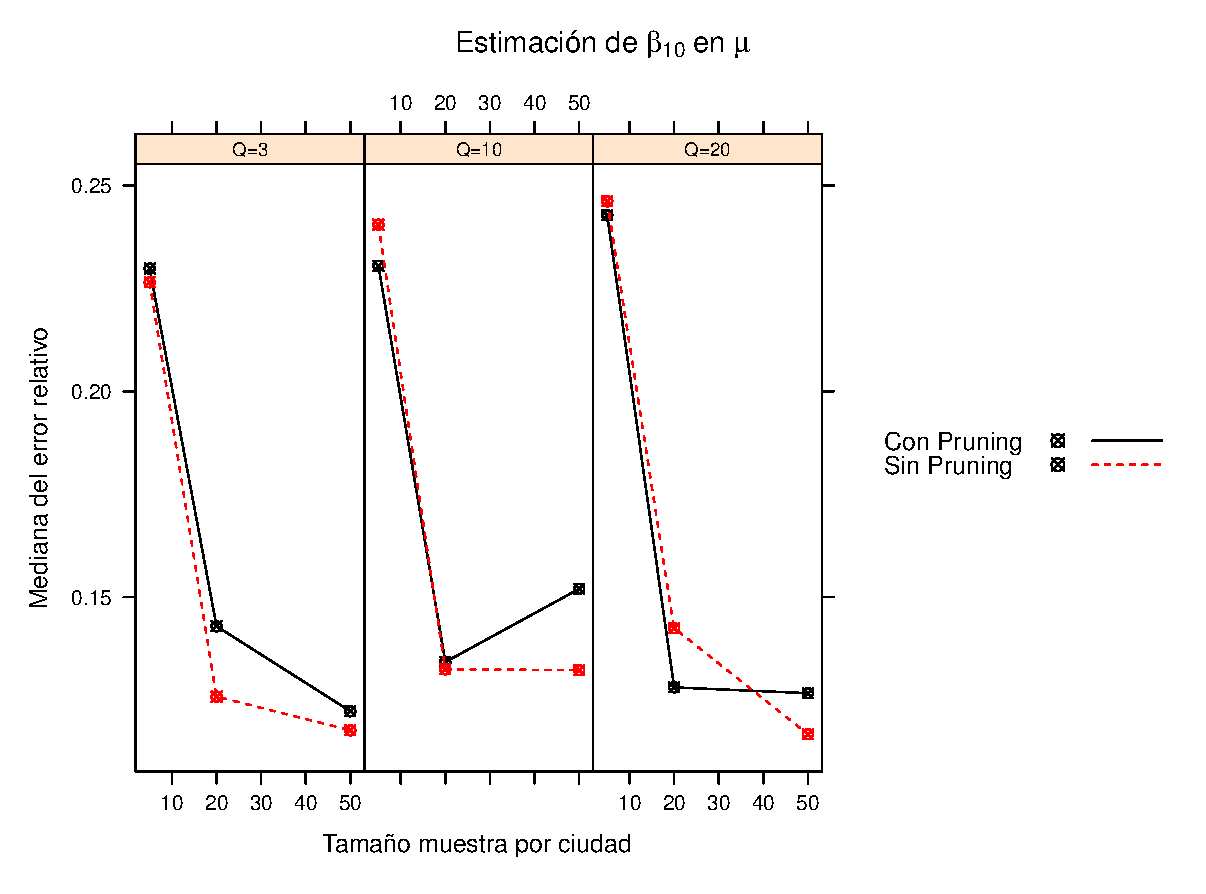
\includegraphics[scale=0.6]{MAPE_beta0_mu.eps}	
		\caption{Anadir}
		\label{MAPE_bo_mu}
	\end{center}
\end{figure}

\begin{figure}
	\begin{center}
		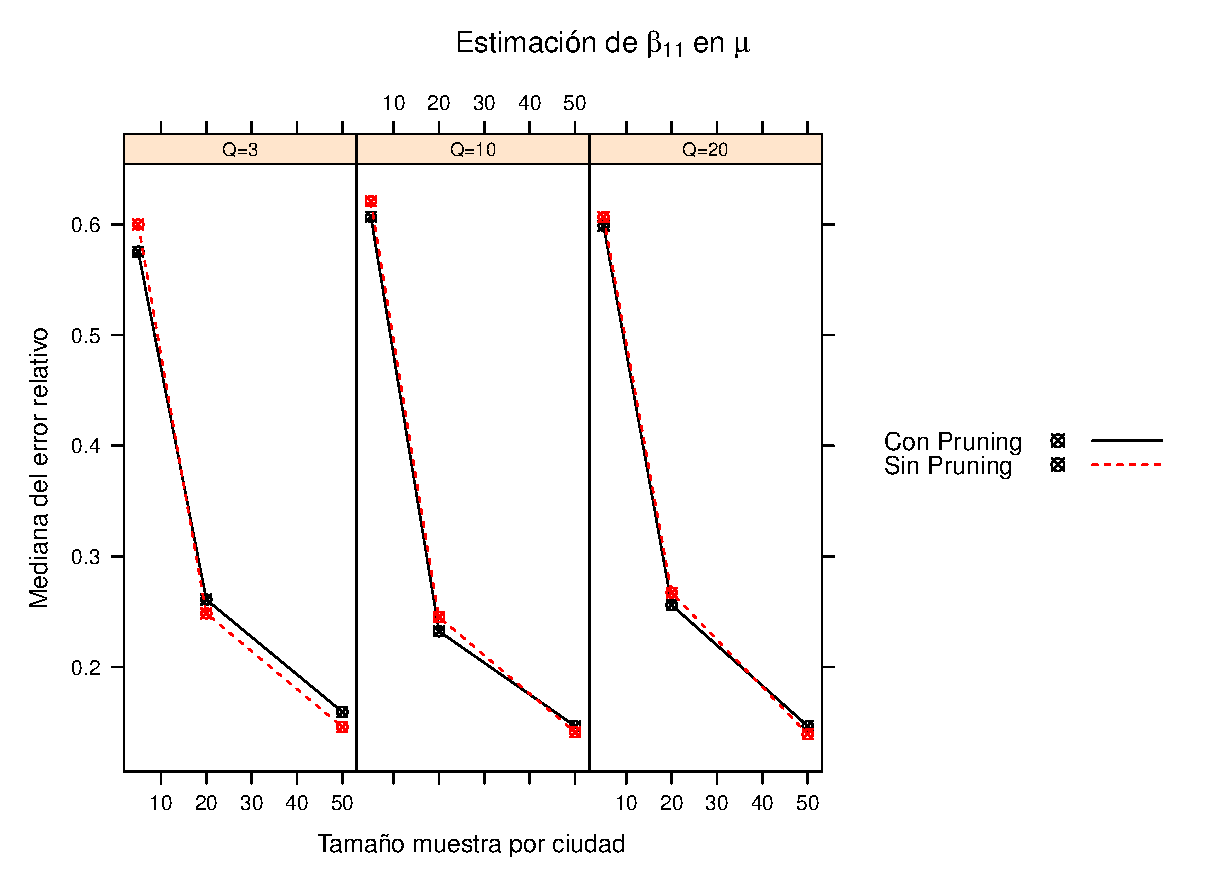
\includegraphics[scale=0.6]{MAPE_beta1_mu.eps}	
		\caption{Anadir}
		\label{MAPE_beta1_mu}
	\end{center}
\end{figure}

\begin{figure}
	\begin{center}
		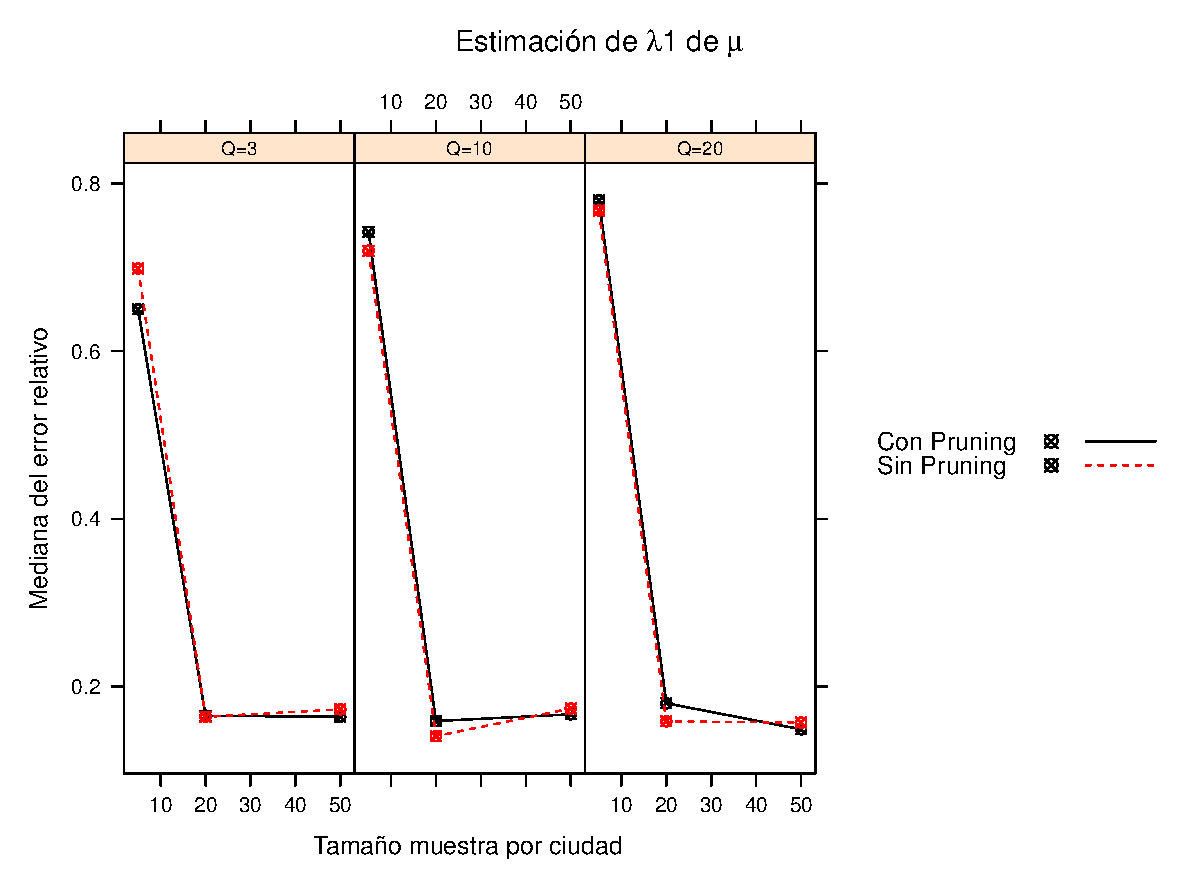
\includegraphics[scale=0.6]{MAPE_lambda1_mu.eps}	
		\caption{Anadir}
		\label{MAPE_lambda1_mu}
	\end{center}
\end{figure}

\begin{figure}
	\begin{center}
		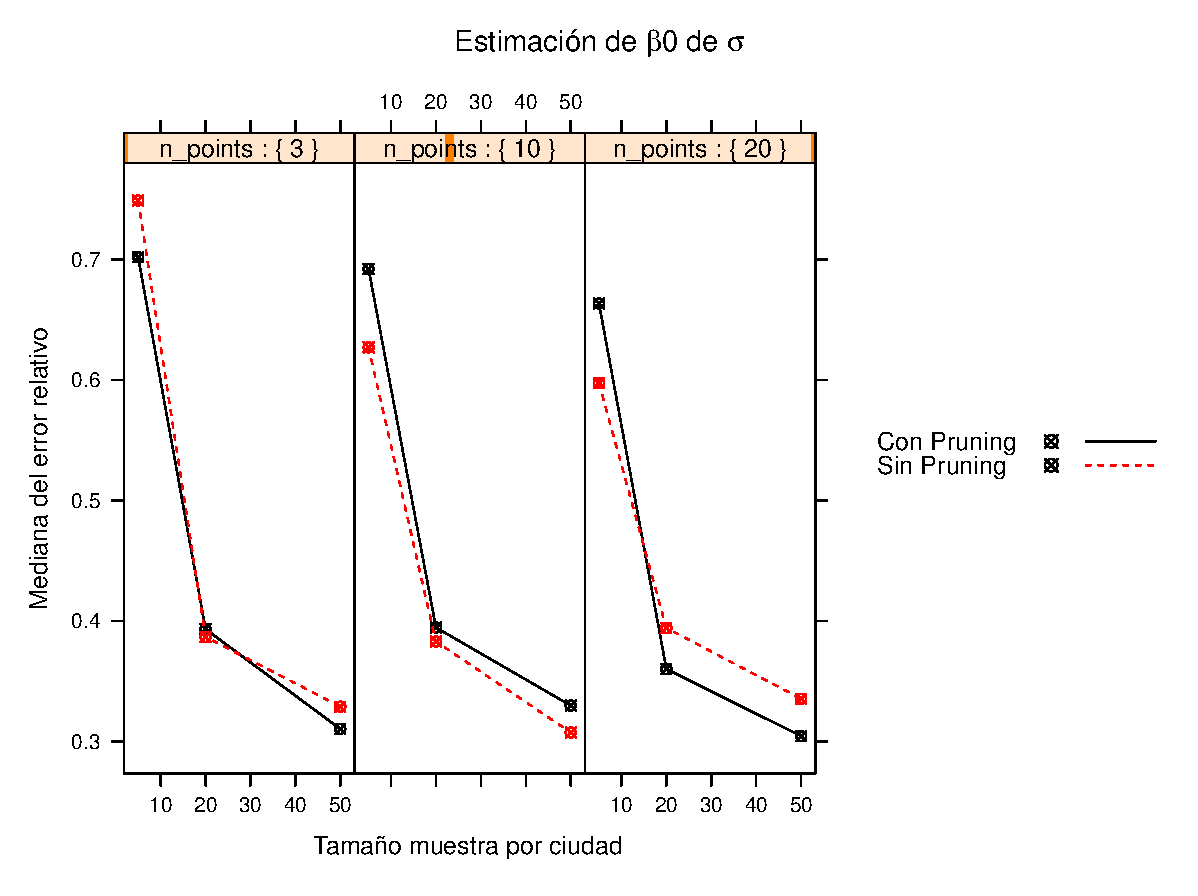
\includegraphics[scale=0.6]{MAPE_beta0_sigma.eps}	
		\caption{Anadir}
		\label{MAPE_beta0_sigma}
	\end{center}
\end{figure}

\begin{figure}
	\begin{center}
		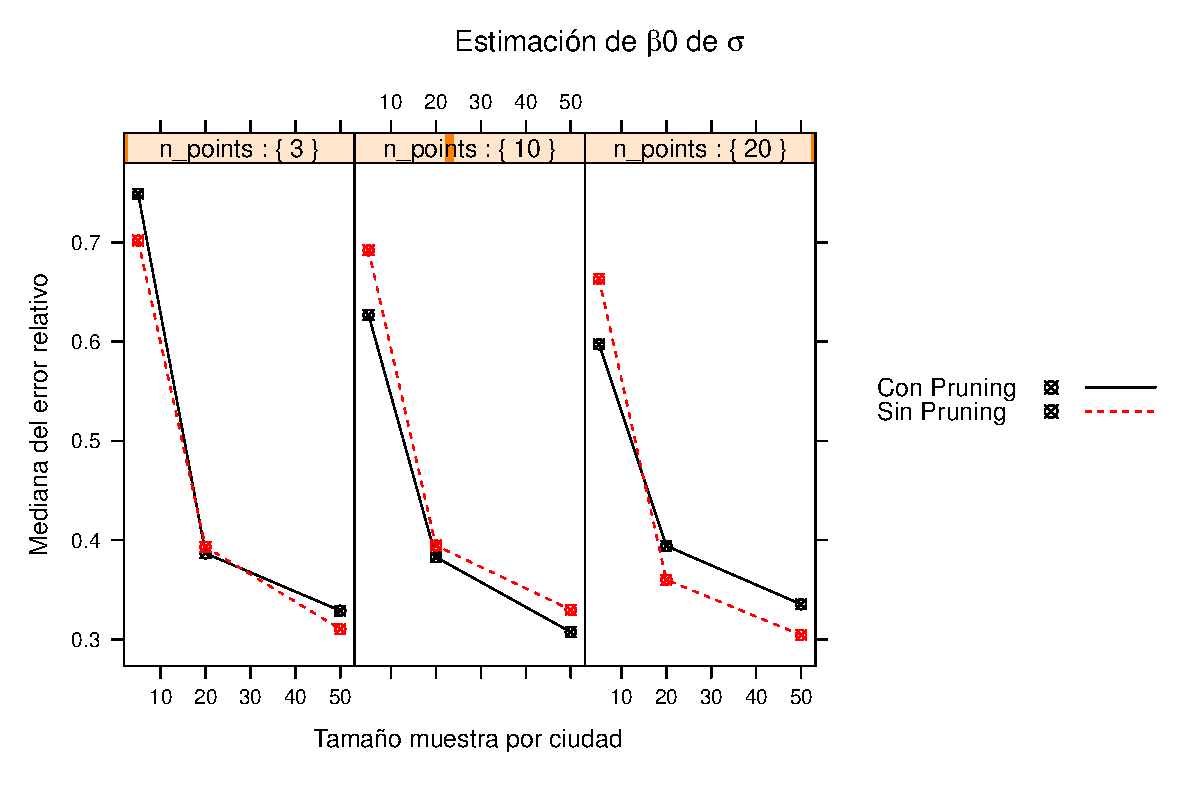
\includegraphics[scale=0.6]{MAPE_beta1_sigma.eps}	
		\caption{Anadir}
		\label{MAPE_beta1_sigma}
	\end{center}
\end{figure}

\begin{figure}
	\begin{center}
		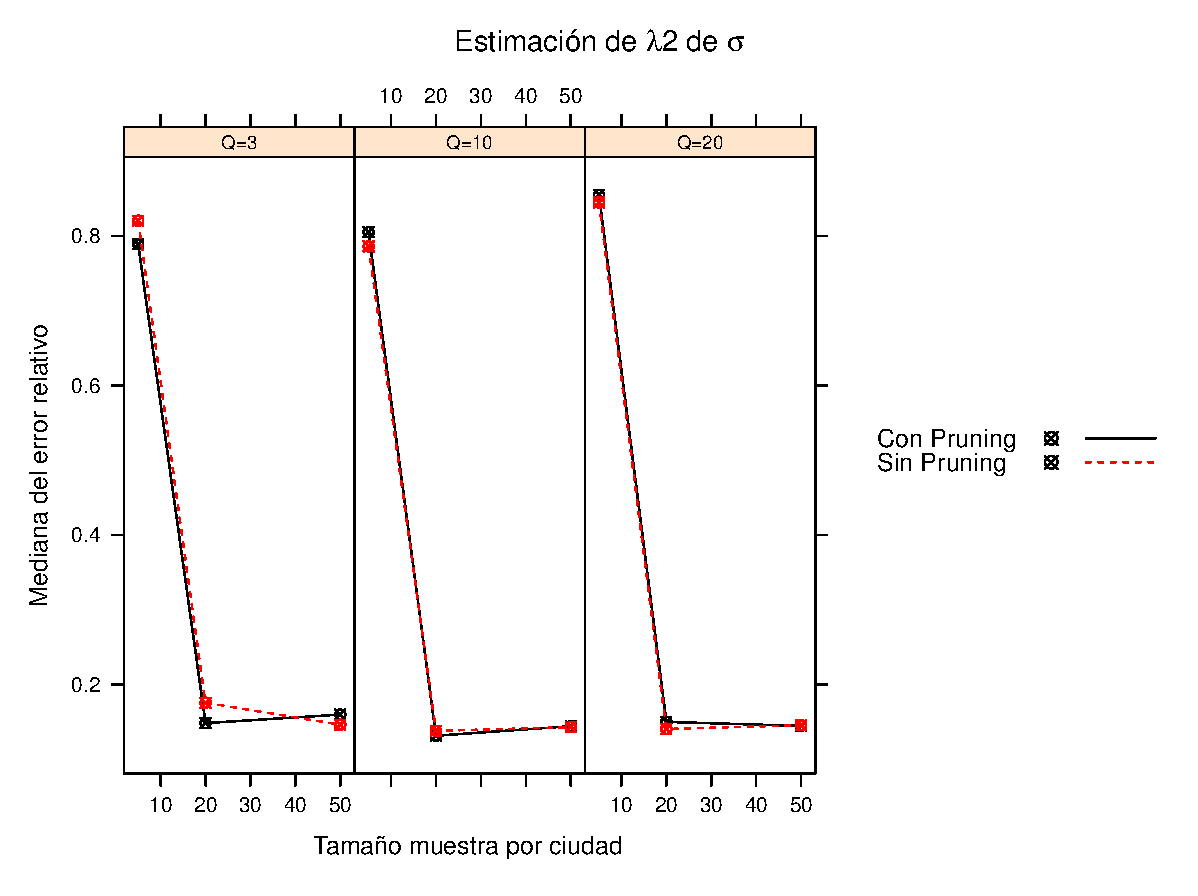
\includegraphics[scale=0.6]{MAPE_lambda2_sigma.eps}	
		\caption{Anadir}
		\label{MAPE_lambda2_sigma}
	\end{center}
\end{figure}

\begin{figure}
	\begin{center}
		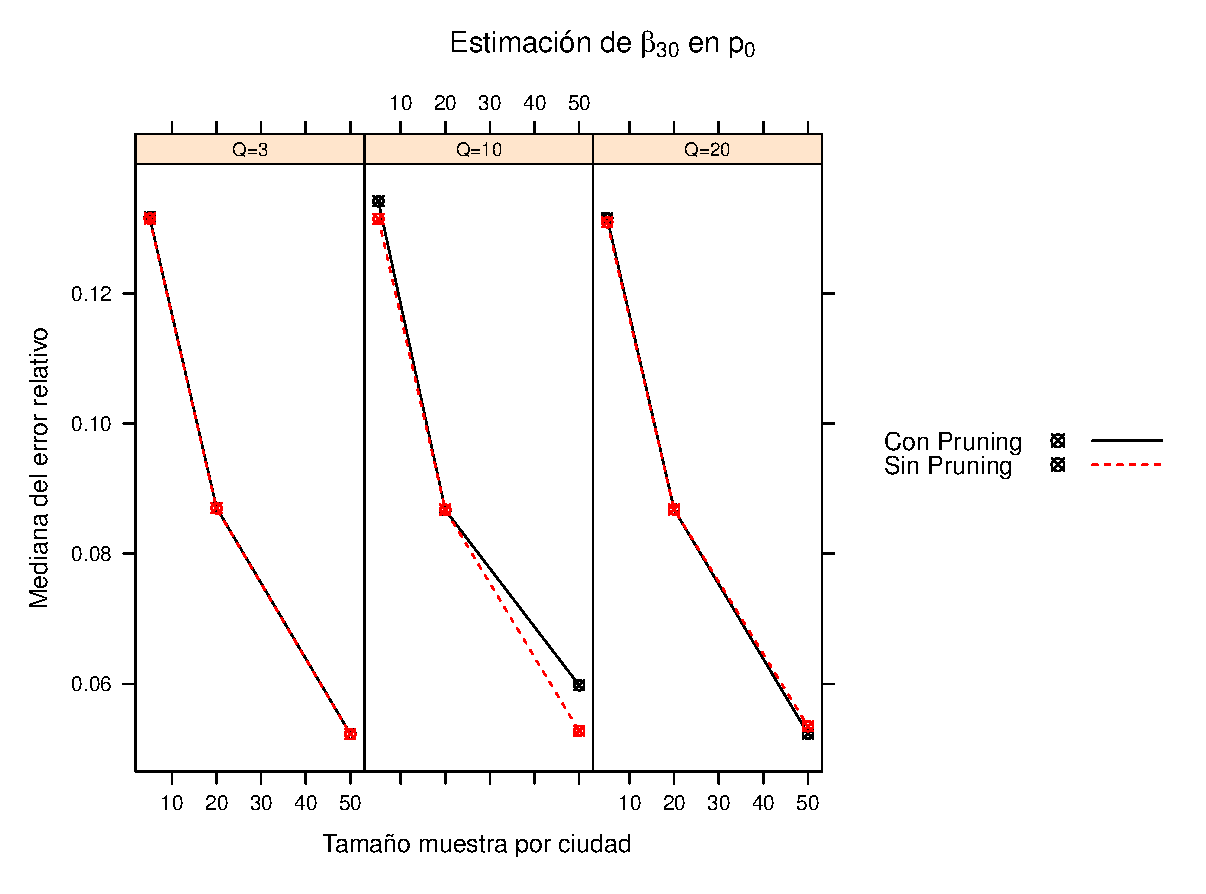
\includegraphics[scale=0.6]{MAPE_beta0_p0.eps}	
		\caption{Anadir}
		\label{MAPE_beta0_p0}
	\end{center}
\end{figure}

\begin{figure}
	\begin{center}
		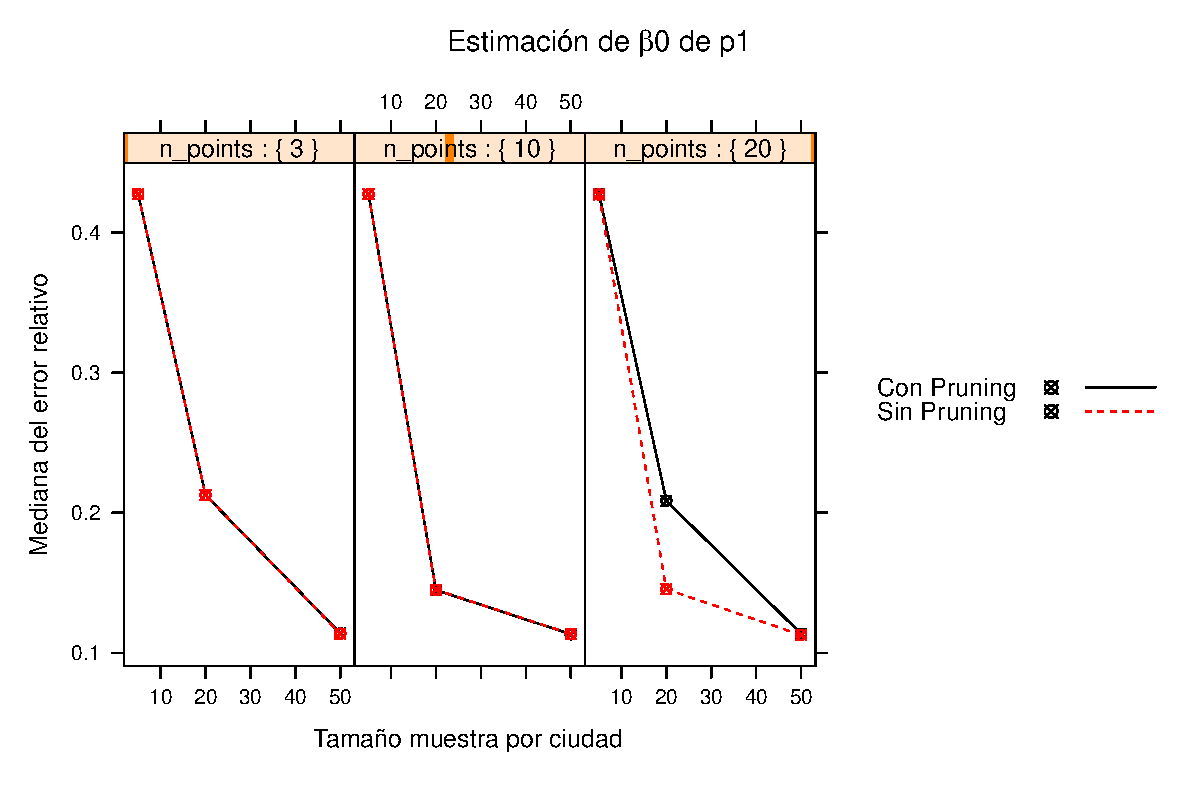
\includegraphics[scale=0.6]{MAPE_beta0_p1.eps}	
		\caption{Anadir}
		\label{MAPE_beta0_p1}
	\end{center}
\end{figure}

\begin{figure}
	\begin{center}
		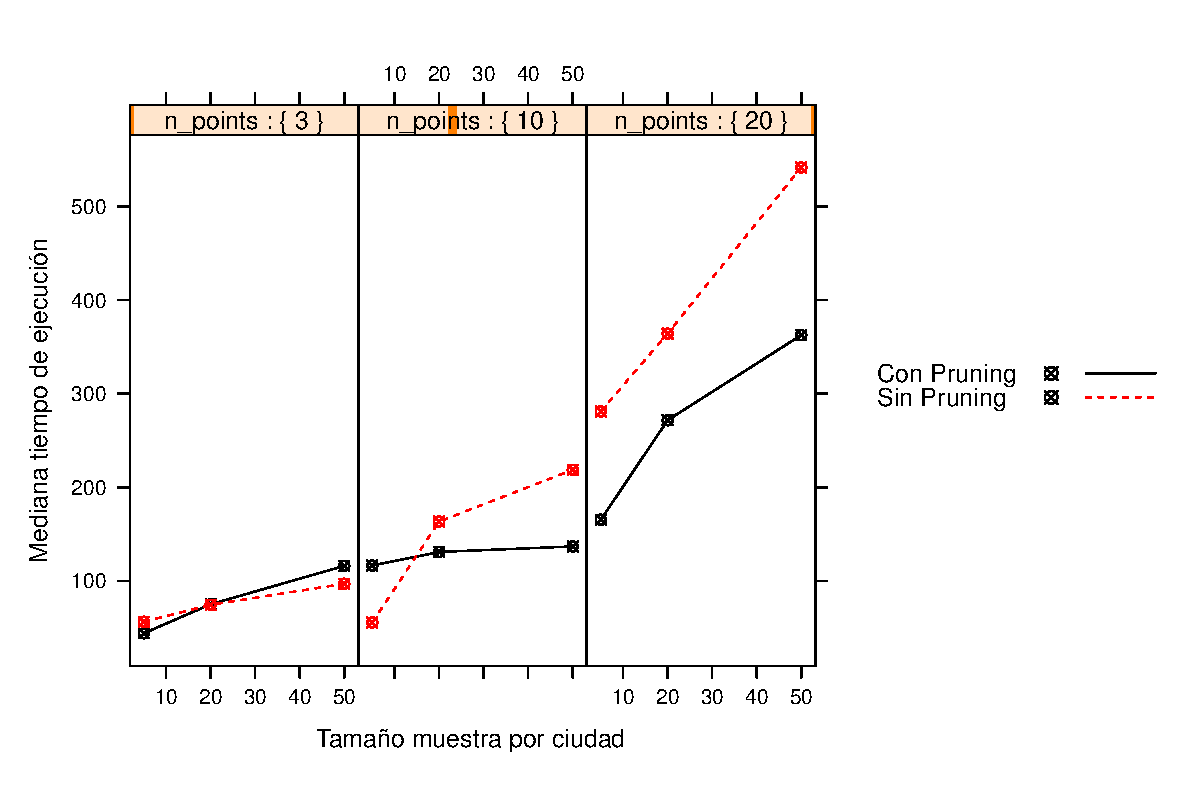
\includegraphics[scale=0.6]{time_mix_ZOIP.eps}	
		\caption{Anadir}
		\label{time_mix_ZOIP}
	\end{center}
\end{figure}

